\chapter{Design}
\label{ch:design}

% In this chapter, we describe the overall design of our solution to the problem identified in \Cref{ch:introduction}, building on work described in \Cref{ch:background}.
% Figure~\ref{fig:topview} shows the top view of the project with modules interconnected.
% \begin{figure*}[t!]
% \begin{figure*}[h]
% \centering
%   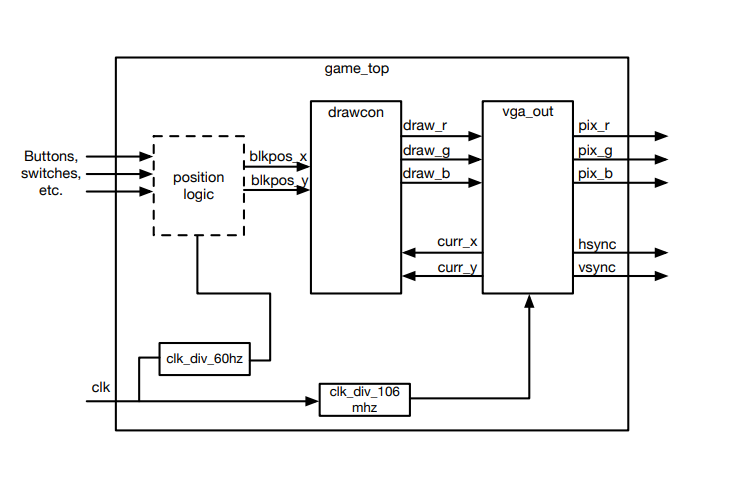
\includegraphics[width=0.8\textwidth,keepaspectratio]{../figures/modules overview.png}
%   \caption{Block diagram of the proposed triple-core lockstep technique (TCLS)}
% \label{fig:topview}
% \end{figure*}
\section{程序架构简介}

在程序设计上,主要实现了以下几个class及成员函数.
\begin{itemize}
  \item TimeIntegrator类: 所有story中微分方程的求解器的基类
  \subitem virtual initialize：主要是根据阶数或者state数(Gauss Legendre RK Methods)来初始化参数
  \subitem virtual solve：求解函数，第一个参数是初值，第二个参数是$u(t)'=f(u,t)$的右侧函数，第三个参数是stepnumber(在自适应步长的方法中实际上只决定第一步的步长)，第四个参数是开始时间，第五个参数是结束时间
  \subitem output：将求解结果输出到文件，第一个参数输出文件路径及文件名，不存在的文件夹会被自动创建，第二个参数是输出后是否清除储存的解(减小内存消耗)的bool变量，第三个参数是输出到文件的形式为添加还是覆写(app还是out)
  \item TimeIntegratorFactory类: 管理求解器的工厂，是一个单例的类
  \subitem registerTimeIntegrator：注册求解器，第一个参数为求解器名,第二个参数是返回指向对应求解器类的unique\_ptr<TimeIntegrator>的右侧函数
  \subitem createTimeIntegrator：根据求解器名创建求解器，第一个参数为求解器名，第二个参数为阶数（主要对于Gauss Legendre RK方法之外的固定步长方法）或者state数（对于Gauss Legendre RK方法）,自适应步长方法和Euler方法随意
  \subitem getInstance：获取求解器工厂的唯一实例
  \item TimeIntegrator的派生类
  \subitem Adama\_Bashforth\_Methods： 对应求解器名Adams-Bashforth
  \subitem Adams\_Moulton\_Methods：对应求解器名Adams-Moulton
  \subitem Backward\_Differentiation\_Formula：对应求解器名Backward\_Differentiation
  \subitem ClassicalRK：对应求解器名ClassicalRK
  \subitem ESDIRK：对应求解器名ESDIRK
  \subitem GLRK：对应求解器名GLRK
  \subitem FhelbergRK：对应求解器名FehlbergRK
  \subitem Dormand\_PrinceRK：对应求解器名Dormand-PrinceRK
  \subitem Euler\_Meythod：对应求解器名Euler
  \item testsolver函数：测试求解器在story问题下的求解，对于固定步长方法，使用二分法寻找10000000步内的使得误差的max-norm小于0.001的最小cputime，对于所有方法的所有阶数的求解器，在步数为1000，10000，100000，1000000步情况下求解story中问题（对于自适应步长方法，实际上只有初始步长受影响）。
  第一个参数为求解器名，第二、三个参数为初始化时order或state number的最小值和最大值。
  \item outputcapture函数：获取输出到终端的内容并输出到txt文件内，第一个参数是txt文件地址，为创建的文件夹会自动创建，第二、三、四个参数为testsolver的参数，第三个参数为函数（实际上输入testsolver）。
  \item UnitTimer类：给程序运行的cpu时间记时
  \subitem begin: 第一个参数为task名称，开始这个task的计时
  \subitem end: 第一个参数为task名称，结束这个task的计时
  \subitem getTime: 第一个参数为task名称，输出该task的cpu时间
  \subitem reset：清除所有计时器
  \subitem report：在终端打印所有task的时间以及程序运行总时间
  \subitem getInstance：获取计时器的唯一实例
  \item VectorFunction类：向量函数类，有重载括号运算符的虚函数，其第一个参数是$u'(t)=f(u,t)$中的$u(std::vector<double>)$,第二个参数是$t(double)$;对于某些求解器，需要正确设定其dim值(即$u$的维数)。
\end{itemize}

\section{程序使用简介}
\subsection{获取story数据}
\begin{verbatim}
StoryFunction storyfunc;
const VectorFunction* func = &storyfunc;
\end{verbatim}
注意StoryFunction已经定义在VectorFunction.h中，表示story中的$f(u,t)$。

\subsection{求解器使用}
\begin{verbatim}
std::unique_ptr<TimeIntegrator> solver = TimeIntegratorFactory::getInstance()
.createTimeIntegrator("classicalRK", 4);\\创建求解器
solver->solve(initial_values,func,100000,0.0,T_1);\\求解
solver->output("output/.../ClassicalRK_100000.txt");\\输出
\end{verbatim}

\subsection{计时器使用}

\begin{verbatim}
UnitTimer& timer=UnitTimer::getInstance();\\获取计时器的唯一实例
timer.reset();\\清空计时器
timer.begin("task1");\\开始计时
timer.end("task1");\\结束这个task的计时
std::cout<<timer.getTime("task1")<<std::endl\\输出该task的cpu时间
timer.report();\\在终端打印所有task的时间以及程序运行总时间
\end{verbatim}

\subsection{产生log}
\begin{verbatim}
outputcapture("../log/Adams-Bashforth.txt",func,...(args of func));
\end{verbatim}

\subsection{绘图}
\begin{verbatim}
python plot/plot.py 
#将output/track文件夹下每个最深层子文件夹的数据绘成一幅图
#将output/acc文件夹下每个文件绘成一幅图
\end{verbatim}

img/acc下每一个文件储存了每个求解器不同阶数在1000，10000，100000，1000000作为step数时求解的误差的最大范数，
绘图逻辑是将1000的误差除以10000的误差然后对10取对数获得一个点，对于其它情况类似。然后将每阶的对应的点连成一条折线。
